\documentclass[submission,copyright,creativecommons,sharealike,noncommercial]{eptcs}
\providecommand{\event}{Working paper}
\pdfoutput=1

%%%% packages.tex by Stefano Gogioso 
%%%% Version 7 Dec 2016

\usepackage[toc,page]{appendix}
%% MATHS %%
\usepackage{mathtools} % Loads and extends amsmath
\usepackage{amssymb} % Extra mathematical symbols (loads amsfonts)
\usepackage{amsthm} % Theorem environments
\usepackage{stmaryrd} % Some maths symbols for logic and computer science
%\usepackage{cjhebrew} % Jewish symbols
%\usepackage[nodisplayskipstretch]{setspace} % Redefines spacing before/after equations

%% WRITING %%
\usepackage{relsize} % Additional relative sizes for fonts
\usepackage{microtype} % Improves appearance of writing
%\usepackage{fullpage} % Reduces lateral page margins for vanilla classes
\usepackage{multicol} % Multi-column environments
\usepackage{csquotes} % Environments for quotes
\usepackage{xspace}
%% CITATIONS %%
%\usepackage{hyperref} % Hyperlink citations, comment out for arxiv submission 
\usepackage[nocompress]{cite} % Comment out if using natbib or apacite
\usepackage[hyperpageref]{backref} 
\renewcommand*{\backref}[1]{}
\renewcommand*{\backrefalt}[4]{%
	\ifcase #1 (Not cited.)%
	\or        (Cited on page~#2.)%
	\else      (Cited on pages~#2.)%
	\fi}
% QPL wants Bibtex!
%\usepackage[
%backend=biber,
%natbib=true,
%language=auto,
%style=numeric-comp,
%sorting=nyt,
%maxbibnames=10,
%firstinits=true,
%url=true, 
%doi=false,
%isbn=false,
%eprint=false
%]{biblatex}

%\usepackage[sort&compress]{natbib} % Comment out if using cite or apacite
%\usepackage[round,authoryear,sort&compress]{natbib} % Comment out if using cite or apacite
%\usepackage{apacite} % Comment out if using natbib or cite

%% GRAPHICS %%
\usepackage{graphicx} % Import of graphics
\usepackage{subcaption} % Captioning and referencing sub-figures
\usepackage{wrapfig} % Figures wrapped in text
\usepackage[usenames,dvipsnames]{xcolor} % Introduces colour names
\usepackage{tikz} % TikZ
\usetikzlibrary{
	math,
	decorations.markings,
	positioning,
  arrows,
  intersections,
%	arrows.meta,
  shapes,
  shapes.misc,
	automata,
	petri,
	decorations,
	backgrounds,
	calc,
	fit,
	quotes
  }

  \usepackage{circuitikz}
%%%% macros.tex by Stefano Gogioso
%%%% Version 12 Apr 2017 


%% Theorem environments - Comment out for certain journal submissions and for beamer 
	%% Counters and miscellaneous
  \newcounter{theoremUnified} % Unified coutner for all theorem environments
  \def\thetheoremUnified{\arabic{section}} % Needed to have counters going with sections
  \numberwithin{theoremUnified}{section} % Numbering within sections
  \numberwithin{theoremUnified}{section} % Equations are also numbered within sections

% Theorem Styles
%
  \newtheoremstyle{plainStyle} % Plain theorem style
  {2mm} % Space above
  {2mm} % Space below
  {} % Body font
  {} % Indent amount
  {\bfseries} % Theorem head font
  {.} % Punctuation after theorem head
  {.5em} % Space after theorem head
  {} % Theorem head spec (can be left empty, meaning `normal')

  \newtheoremstyle{italicStyle} % Italic theorem style
  {2mm} % Space above
  {2mm} % Space below
  {\itshape} % Body font
  {} % Indent amount
  {\bfseries} % Theorem head font
  {.} % Punctuation after theorem head
  {.5em} % Space after theorem head
  {} % Theorem head spec (can be left empty, meaning `normal')

% Ubiquitous set names
\newcommand{\Naturals}{\mathbb{N}} % Set of natural numbers
\newcommand{\Integers}{\mathbb{Z}} % Set of interer numbers
\newcommand{\Bool}{\mathbb{B}} % Set of interer numbers

% Background for tikz images
\def\backgrnd{black!10}	% Background for Tikz pictures

% Basic Definitions
%
\newcommand{\Obj}[1]{\operatorname{Obj} \, #1} % Set of objects of category #1
\newcommand{\Mor}[1]{\operatorname{Mor} \, #1} % Set of objects of category #1
\newcommand{\GObj}[1]{\operatorname{GenObj} \, #1} % Set of objects of category #1
\newcommand{\GMor}[1]{\operatorname{GenMor} \, #1} % Set of objects of category #1

\newcommand{\Snark}[1]{\operatorname{Sn}(#1)} % Set of objects of category #1

\newcommand{\Homtotal}[1]{\operatorname{Hom}_{\,#1}} % Set of morphisms of category #1
\newcommand{\Hom}[3]{\operatorname{Hom}_{\,#1}\left[#2,#3\right]} % Set of morphisms of category #1 from object #2 to object #3
\newcommand{\Source}[2]{\operatorname{s}_{#1}(#2)} % Domain of function/morphism #1
\newcommand{\Target}[2]{\operatorname{t}_{#1}(#2)} % Domain of function/morphism #1
\newcommand{\Id}[1]{id_{#1}} % Identity morphism of object #1

% Generic names for categories
%
\newcommand{\CategoryA}{\mathcal{A}}
\newcommand{\CategoryB}{\mathcal{B}}
\newcommand{\CategoryC}{\mathcal{C}}
\newcommand{\CategoryD}{\mathcal{D}}
\newcommand{\CategoryE}{\mathcal{E}}

\newcommand{\Free}[1]{\mathfrak{F}(#1)}
\newcommand{\UnFree}[1]{\mathfrak{U}(#1)}

% Monoidal Categories
%
\newcommand{\Tensor}{\otimes} % Monoidal tensor
\newcommand{\TensorUnit}{I} % Monoidal tensor unit

% Logic
%
\newcommand{\Suchthat}[2]{\left\{#1 \: \middle\vert \: #2\right\}} % Set of elements #1 such that condition #2 holds 

% Category Names
\newcommand{\Bfun}{\Bool_\textbf{fun}} % Category of boolean functions
\newcommand{\Bcirc}{\Bool_\textbf{circ}} % Category of boolean circuits
\newcommand{\Bkp}{\Bool_\textbf{KP}} % Category of KP boolean circuits
\newcommand{\Bzkp}[1]{\Bool^{#1}_{\textbf{ZKP}}} % Category of KP boolean circuits

\newcommand{\Bpath}[1]{\Bool^{#1}_{\textbf{path}}} % Category of path proofs
\newcommand{\Count}{\textbf{Count}} % Category of KP boolean circuits
\newcommand{\Bgraph}[1]{\Bool^{#1}_{\Graph}} % Category of proof for a whole automaton
\newcommand{\Bsnark}{\Bool_\textbf{SNARK}} % Category of snark boolean circuits
\newcommand{\BsnarkSize}[1]{\Bool^{#1}_{\textbf{path}}} % Category of full snark proofs of some computational size

\newcommand{\Graph}{\textbf{Graph}} % Category of graphs
\newcommand{\Cat}{\textbf{Cat}} % Category of graphs

\newcommand{\NAND}{\ensuremath{\texttt{NAND}}\xspace}
\newcommand{\AND}{\ensuremath{\texttt{AND}}\xspace}
\newcommand{\NOT}{\ensuremath{\texttt{NOT}}\xspace}
\newcommand{\OR}{\ensuremath{\texttt{OR}}\xspace}
\newcommand{\XOR}{\ensuremath{\texttt{XOR}}\xspace}
\newcommand{\COPY}{\ensuremath{\texttt{COPY}}\xspace}
\newcommand{\TRUE}{\ensuremath{\texttt{TRUE}}\xspace}
\newcommand{\FALSE}{\ensuremath{\texttt{FALSE}}\xspace}
\newcommand{\Zero}{\ensuremath{\textbf{0}}\xspace}


\newcommand{\NANDSym}{
  \scalebox{0.3}{
    \tikz[baseline=-10pt] \node[thick, american nand port] (char) {};
  }
}

\newcommand{\XORSymb}{
  \scalebox{0.3}{
    \tikz[baseline=-10pt] \node[thick, american xor port] (char) {};
  }
}

\newcommand{\ANDSym}{
  \scalebox{0.3}{
    \tikz[baseline=-10pt] \node[thick, american and port] (char) {};
  }
}

\newcommand{\ORSym}{
  \scalebox{0.3}{
    \tikz[baseline=-10pt] \node[thick, american or port] (char) {};
  }
}
\newcommand{\COPYSym}{
  \scalebox{0.3}{
    \tikz[baseline=-8pt]{
      \node[thick, draw, circle, radius=2pt] (copy) at (0,0) {};
      \node (in) at (-1,0) {};
      \node (out1) at (1,0.5) {};            
      \node (out2) at (1,-0.5) {};
      \draw[thick, -] (in.center) to (copy);
      \draw[thick, -, bend left] (copy) to (out1.center);
      \draw[thick, -, bend right] (copy) to (out2.center);
    } 
  }
}

\newcommand{\MATCHSym}{
  \scalebox{0.3}{
    \tikz[baseline=-8pt]{
      \node[thick, draw, fill=gray, circle, radius=2pt] (copy) at (0,0) {};
      \node (in) at (1,0) {};
      \node (out1) at (-1,0.5) {};            
      \node (out2) at (-1,-0.5) {};
      \draw[thick, -, dotted] (in.center) to (copy);
      \draw[thick, -, bend right] (copy) to (out1.center);
      \draw[thick, -, bend left] (copy) to (out2.center);
    } 
  }
}

\tikzstyle{place}=
[circle,thick,draw=blue!75,fill=blue!20,minimum size=6mm]
\tikzstyle{transition}=
[rectangle,thick,draw=black!75,fill=black!20,minimum size=4mm]


% QPL wants Bibtex! \addbibresource{Bibliography.bib}


% Macros for coloured text comments.
% Example usage: \commentFG{This is a comment.}{19 Dec}
\newcommand{\commentFG}[2]{\textcolor{blue}{#1 [FG on #2]}}
\newcommand{\commentJH}[2]{\textcolor{red}{#1 [JH on #2]}}
\newcommand{\margincomment}[2]{\marginpar{\tiny\color{#1}#2}}
\newcommand{\marginFG}[1]{\margincomment{blue}{#1}}
\newcommand{\marginJH}[1]{\margincomment{red}{#1}}

\setcounter{tocdepth}{2}

\title{Mapping finite state machines to zk-SNARKS \\ Using Category Theory}
\author{
	F. Genovese, A.Knispel, J. Fitzgerald \\
	Statebox Team\\
	\texttt{research@statebox.io}
}

\def\titlerunning{Mapping finite state machines to zk-SNARKS}
\def\authorrunning{F. Genovese, A.Knispel \& J. Fitzgerald}


\begin{document}
\maketitle
%
%
\begin{abstract}
  We provide a categorical procedure to turn graphs corresponding to 
  state spaces of finite state machines into boolean circuits, leveraging on the fact that 
  boolean circuits can be easily turned into zk-SNARKS. Our 
  circuits verify that a given sequence of edges and nodes is indeed a 
  path in the graph they represent. We then generalize to circuits verifying 
  paths in arbitrary graphs. We prove that all of our correspondences are 
  pseudofunctorial, and behave nicely with respect to each other.
\end{abstract}
%
%
%
\section{Introduction}\label{sec:introduction}
%
%
Lately, especially due to the advent of smart contracts 
in business applications, there has been a renewed interest towards 
classical results in theoretical computer science.

Smart contracts, especially if hosted on the blockchain~[], are immutable
pieces of code, more often than not used to manage money. These are 
very good reasons to look into ways of writing smart contracts  
that are reliable, easy to analyze and correct-by-construction. These requirements
 renewed interest in formal models of computation~[]: In particular, 
 \emph{finite state machines (FSMs)}~[] are considered easy 
 to implement, well structured, and make possible to prove 
 roperties of the computations being performed. 

On the other hand, blockchain also spawned a renewed interest for 
cyptography, both for security, privacy, and space reasons: It is 
paramount for blockchains to be cryptographically secure, if they are 
meant to work as exchanges of valuables of any sort (such as digital currency).
As for privacy, cryptographic tools such as \emph{zero-knowledge 
succinct non-interactive argument of knowledge (zk-SNARKS)}~[] allow for 
the verification that an information is correct without actually revealing anything
about the information itself. This has been used, for instance, by ZCash~[] to 
implement private blockchain transactions: Here, transacting parties submit 
zk-SNARKs of their transactions to the blockchain, and miners then verify that a given 
transaction followed the rules of the protocol by verifying the zk-SNARK, 
without gaining any information about who-sent-money-to-who, and 
how much. 
Regarding space, it has to be noted that by design blockchains tend to 
grow indefinitely space-wise as new blocks keep being added to the chain. 
This is a serious issue, since new nodes are either forced to download many 
gigabytes of data to sync with the network or they have to require the current state 
of the chain from another node (which requires trusting the node) and then start 
syncing from there. This ``trust vs. feasibility'' issue can be resolved by \emph{recursive 
zk-SNARKS}~[], in which are used to verify, using just a few Kbs, that the current 
state received by a node is valid. Such applications look very promising especially in 
contexts such as blockchain applied to the Internet of Things~[].

In this work, we put together formal models of computation and 
cryptography, providing a categorical way to turn finite state machines into zk-SNARKs 
that verify how a sequence of inputs leading to a state change follows the 
rules specified by the finite state machine itself. To do this, we bypass the problem 
of modelling cryptographical primitives categorically, using the 
fact that boolean circuits can be easily turned into zk-SNARKS by already 
available techniques. 

We proceed as follows: In Section~\ref{sec: the categories bfun, bcirc, bkp} we 
define boolean circuits from a categorical perspective. 
In Section~\ref{sec: finite state machines} we briefly 
explain the links between finite state machines and free categories. 
In Section~\ref{sec: turning executions into circuits} 
we show how to turn a given sequence of state changes 
for a given finite state machine into a boolean circuit. We then obtain a 
generalized boolean circuit which verifies arbitrary sequences up to 
a given length, and show how it can be turned into a zk-SNARK. 
In Section~\ref{sec: abstracting over graphs} we generalize to 
circuits which accept the specification defining a finite state machine 
as input, thus attaining full privacy. In Section~\ref{sec: conclusion} 
we conclude by defining directions of future work.

\section[The categories Bfun, Bcirc, Bkp]{The categories $\Bfun$, $\Bcirc$, $\Bkp$}
\label{sec: the categories bfun, bcirc, bkp}
%
%
\begin{definition}
  A \emph{boolean function} is a function $\Bool^n \to \Bool$,
  for some natural $n$. A \emph{generalized boolean function} 
  is a function $\Bool^n \to \Bool^m$, for naturals $m, n$.
  We denote with $\Bfun$ \emph{the category of generalized 
  boolean functions}, having $\Bool^n$, for each natural $n$ as objects,
  and generalized boolean functions as morphisms. Composition is 
  the usual function composition. This category 
  is clearly symmetric monoidal, with $\Bool^0$ as unit, 
  and the usual product of functions as product.
\end{definition}
%
%
\begin{definition}
  A \emph{boolean circuit} is a wiring of logical gates that computes a 
  boolean function $\Bool^n \to \Bool$. A \emph{generalized boolean 
  circuit} is a wiring of logical gates that computes a generalized boolean 
  function $\Bool^n \to \Bool^m$.
  We denote with $\Bcirc$ \emph{the category of generalized boolean circuits}, 
  that is, the free symmetric strict monoidal category generated by one object, 
  denoted with $X$, and the following four morphisms:
  %
  %
  \begin{equation*}
    \tikz[baseline]{
      \node[american nand port] (nand) at (1.5,0) {};
      \node at ([xshift=5pt]nand.out) {$X$};
      \node at (0,0.3) {$X$} ;
      \node at (0,-0.3) {$X$} ;
    }
    \qquad\qquad
    \tikz[baseline]{
      \node[thick, draw, circle, radius=2pt] (copy) at (0,0) {};
      \node[label={[label distance=-10pt]180:$X$}] (in) at (-1,0) {};
      \node[label={[label distance=-10pt]0:$X$}]  (out1) at (1,0.5) {};            
      \node[label={[label distance=-10pt]0:$X$}]   (out2) at (1,-0.5) {};
      \draw[thick, -] (in) to (copy);
      \draw[thick, -, bend left] (copy) to (out1);
      \draw[thick, -, bend right] (copy) to (out2);
    }
    \qquad\qquad
    \tikz[baseline]{
      \node[thick, draw, circle, radius=2pt, inner sep = 2pt] (true) at (0,0) {\tiny{$\top$}};
      \node[label={[label distance=-10pt]0:$X$}] (out) at (1,0) {};        
      \draw[thick, -] (copy) to (out);
    }
    \qquad\qquad
    \tikz[baseline]{
      \node[thick, draw, circle, radius=2pt, inner sep = 2pt] (true) at (0,0) {\tiny{$\bot$}};
      \node[label={[label distance=-10pt]0:$X$}] (out) at (1,0) {};            
      \draw[thick, -] (copy) to (out);
    }
  \end{equation*}
  %
  Respectively called  \NAND,  \COPY, \TRUE, \FALSE. We will often use $X^n$ 
  to denote the $n$-fold monoidal product of $X$, and $X^0$ to denote the monoidal 
  unit.
  %
  For more information about how to generate a free symmetric strict monoidal 
  category from a set of object and morphism generators, see~[].
\end{definition}
%
As the name suggests, we interpret \NANDSym as the \NAND gate, \COPYSym as 
the gate that copies a bit, and \TRUE and \FALSE as constants. We can reify 
this interpretation using the following lemma:
%
%
\begin{lemma}\label{lem: monoidal functor Bcirc Bfun}
  There is a strict monoidal functor $\texttt{ext}: \Bcirc \to \Bfun$ sending
  $I$ to $\Bool^0$, $X$ to $\Bool$, $\NANDSym$ to the usual 
  \texttt{NAND} function $\Bool^2 \to \Bool$, $\COPYSym$ to the 
  cartesian diagonal on $\Bool$, and $\top, \bot$ to the 
  functions $\Bool^0 \to \Bool$ corresponding to the constants 
  $1$ and $0$, respectively.
\end{lemma}
%
Indeed, there are multiple choices for the generators of $\Bcirc$. We decided to 
use \NAND because it is well known that this gate, along with the possibility to 
copy bits, is enough to generate any $n$-ary logical circuit~[]. In the following, we 
will often refer to other gates, such as $\ORSym$ (called \emph{\OR}) or 
$\ANDSym$ (\emph{\AND}): In our setting, these are just syntactic sugar for the 
opportune wirings of $\NANDSym$ and $\COPYSym$ to simulate them.
%
%
\begin{definition}\label{def: definition of bkp}
  We denote with $\Bkp$ the \emph{bicategory of knowledge proof circuits} defined 
  as follows:
  %
  %
  \begin{itemize}
    \item $\Obj{\Bkp} := \Obj{\Bcirc}$;
    \item $\Mor{\Bkp}(A,B) := \Mor{\Bcirc}(A \Tensor X^n, X \Tensor B )$, for all $n \in \Naturals$.
    We depict morphisms as shown below; the $X^n$ and $X$ wires are ``silent'' with respect to 
    our categorical structure, so we depict them dashed and dotted, respectively:
    %
    %
    \begin{equation*}
    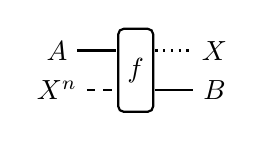
\begin{tikzpicture}
      \node[draw, minimum height=30, minimum width=5, rounded corners=2, thick] (f) at (-1,0.5) {$f$};
      \node (A) at (-2,0.75) {$A$};
      \node (Xn0) at (-2,0.25) {$X^{n}$};
      \node (Bf) at (0,0.75) {$X$};
      \node (B) at (0,0.25) {$B$};

      \draw[thick] (A) -- (-1.25,0.75);
      \draw[dashed,thick] (Xn0) -- (-1.25,0.25);

      \draw[dotted,thick] (-0.75,0.75) -- (Bf);
      \draw[thick] (-0.75,0.25) -- (B);
    \end{tikzpicture}  
    \end{equation*}
    %
    \item $\Id{A} := \top \Tensor \Id{A}: A \Tensor X^0 \to X \Tensor A$. Identites are
    depicted as follows:
    %
    %
    \begin{equation*}
      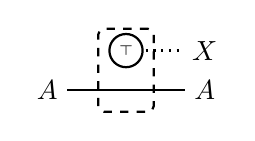
\begin{tikzpicture}
        \node[draw, dashed, minimum height=30, minimum width=20, rounded corners=2, thick] (f) at (-1,0.5) {};
        \node[thick, draw, circle, radius=2pt, inner sep = 2pt] (true) at (-1,0.75) {\tiny{$\top$}};
        \node (A) at (-2,0.25) {$A$};
        \node (Bf) at (0,0.75) {$X$};
        \node (B) at (0,0.25) {$A$};
  
        \draw[thick] (A) -- (B);
  
        \draw[dotted, thick] (-0.75,0.75) -- (Bf);
      \end{tikzpicture}  
      \end{equation*}
      %
    \item $\Mor{\Bkp}(A,B)(f,g) = \begin{cases}
      \{*\} & \text{ iff } \texttt{ext}(f) = \texttt{ext}(g);\\
      \,\,\,\, \emptyset & \text{ otherwise}
    \end{cases}$
    %
    \item Given $f : A \to B$ and $g: B \to C$, corresponding to 
    morphisms of $\Bcirc$ $A \Tensor X^{n_0} \to X \Tensor B$ and 
    $B \Tensor X^{n_1} \to X \Tensor C$, respectively, 
    we set $f;g$ to be the morphism 
    $(f \Tensor \Id{X^{n_1}});(\Id{X} \Tensor g);(\ANDSym \Tensor \Id{C})$.
    Composition is depicted graphically as follows:
    %
    %
    \begin{equation*}
      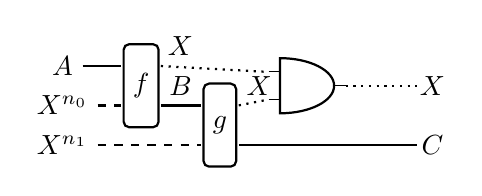
\begin{tikzpicture}
        \ctikzset{tripoles/american and port/input height=0.7};
        \ctikzset{tripoles/american and port/height=.5};
        \ctikzset{tripoles/american and port/width=.7};
        \node[draw, minimum height=30, minimum width=5, rounded corners=2, thick] (f) at (-1,0.5) {$f$};
        \node[draw, minimum height=30, minimum width=5, rounded corners=2, thick] (g) at (0,0) {$g$};
        \node[american and port] (and) at (1.5,0.5) {};

        \node (A) at (-2,0.75) {$A$};
        \node (Xn0) at (-2,0.25) {$X^{n_0}$};
        \node (Xn1) at (-2,-0.25) {$X^{n_1}$};

        \node (Bf) at (-0.5,1) {$X$};
        \node (B) at (-0.5,0.5) {$B$};

        \node (Bg) at (0.5,0.5) {$X$};
        
        \node (X) at (2.7,0.5) {$X$};
        \node (C) at (2.7,-0.25) {$C$};

        \draw[thick] (A) -- (-1.25,0.75);
        \draw[dashed, thick] (Xn0) -- (-1.25,0.25);
        \draw[dashed, thick] (Xn1) -- (-0.24,-0.25);

        \draw[dotted, thick] (-0.75,0.75) -- (and.in 1);
        \draw[thick] (-0.75,0.25) -- (-0.24,0.25);

        \draw[dotted, thick] (0.24,0.25) -- (and.in 2);

        \draw[dotted, thick] (and.out) -- (2.5,0.5);
        \draw[thick] (0.24,-0.25) -- (2.5,-0.25);
      \end{tikzpicture}
    \end{equation*}
    %
    \item The 2-cell compositions and identities are trivial, and defined 
    in the obvious way.
  \end{itemize}
  %
\end{definition}
%
The reason why we define $\Bkp$ as a bicategory is that our 
1-cell composition in $\Bkp$ is not associative. Indeed, $(f;g);h$ and $f;(g;h)$
are different morphisms, as one can see in the figure below:
%
%
\begin{equation*}
  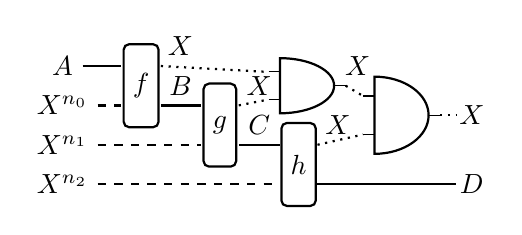
\begin{tikzpicture}
    \ctikzset{tripoles/american and port/input height=0.7};
    \ctikzset{tripoles/american and port/height=.5};
    \ctikzset{tripoles/american and port/width=.7};
    \node[draw, minimum height=30, minimum width=5, rounded corners=2, thick] (f) at (-1,0.5) {$f$};
    \node[draw, minimum height=30, minimum width=5, rounded corners=2, thick] (g) at (0,0) {$g$};
    \node[draw, minimum height=30, minimum width=5, rounded corners=2, thick] (h) at (1,-0.5) {$h$};
    \node[american and port] (and) at (1.5,0.5) {};
    \ctikzset{tripoles/american and port/input height=0.765};
    \ctikzset{tripoles/american and port/height=.7};
    \ctikzset{tripoles/american and port/width=.7};
    \node[american and port] (and2) at (2.7,0.125) {};

    \node (A) at (-2,0.75) {$A$};
    \node (Xn0) at (-2,0.25) {$X^{n_0}$};
    \node (Xn1) at (-2,-0.25) {$X^{n_1}$};
    \node (Xn2) at (-2,-0.75) {$X^{n_2}$};

    \node (Bf) at (-0.5,1) {$X$};
    \node (B) at (-0.5,0.5) {$B$};

    \node (Bg) at (0.5,0.5) {$X$};
    \node (C) at (0.5,0) {$C$};

    \node (Band) at (1.75,0.75) {$X$};
    \node (Bh) at (1.5,0) {$X$};
    \node (Bfin) at (3.2,0.125) {$X$};
    \node (D) at (3.2,-0.75) {$D$};

    \draw[thick] (A) -- (-1.25,0.75);
    \draw[dashed, thick] (Xn0) -- (-1.25,0.25);
    \draw[dashed, thick] (Xn1) -- (-0.24,-0.25);
    \draw[dashed, thick] (Xn2) -- (0.76,-0.75);

    \draw[dotted, thick] (-0.75,0.75) -- (and.in 1);
    \draw[thick] (-0.75,0.25) -- (-0.24,0.25);

    \draw[dotted, thick] (0.24,0.25) -- (and.in 2);
    \draw[thick] (0.24,-0.25) -- (0.76,-0.25);

    \draw[dotted, thick] (and.out) -- (and2.in 1);
    \draw[dotted, thick] (1.24,-0.25) -- (and2.in 2);

    \draw[dotted, thick] (and2.out) -- (3,0.125);
    \draw[thick] (1.24, -0.75) -- (3,-0.75);
  \end{tikzpicture}
  \qquad\qquad
  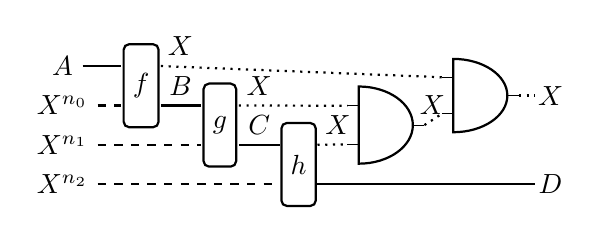
\begin{tikzpicture}
    \node[draw, minimum height=30, minimum width=5, rounded corners=2, thick] (f) at (-1,0.5) {$f$};
    \node[draw, minimum height=30, minimum width=5, rounded corners=2, thick] (g) at (0,0) {$g$};
    \node[draw, minimum height=30, minimum width=5, rounded corners=2, thick] (h) at (1,-0.5) {$h$};
    \ctikzset{tripoles/american and port/input height=0.5};
    \ctikzset{tripoles/american and port/height=.7};
    \ctikzset{tripoles/american and port/width=.7};
    \node[american and port] (and) at (2.5,0) {};
    \ctikzset{tripoles/american and port/input height=0.8};
    \ctikzset{tripoles/american and port/height=.665};
    \ctikzset{tripoles/american and port/width=.7};
    \node[american and port] (and2) at (3.7,0.375) {};

    \node (A) at (-2,0.75) {$A$};
    \node (Xn0) at (-2,0.25) {$X^{n_0}$};
    \node (Xn1) at (-2,-0.25) {$X^{n_1}$};
    \node (Xn2) at (-2,-0.75) {$X^{n_2}$};

    \node (Bf) at (-0.5,1) {$X$};
    \node (B) at (-0.5,0.5) {$B$};

    \node (Bg) at (0.5,0.5) {$X$};
    \node (C) at (0.5,0) {$C$};

    \node (Bh) at (1.5,0) {$X$};
    \node (Band) at (2.7,0.25) {$X$};
    \node (Bfin) at (4.2,0.375) {$X$};
    \node (D) at (4.2,-0.75) {$D$};

    \draw[thick] (A) -- (-1.25,0.75);
    \draw[dashed, thick] (Xn0) -- (-1.25,0.25);
    \draw[dashed, thick] (Xn1) -- (-0.24,-0.25);
    \draw[dashed, thick] (Xn2) -- (0.76,-0.75);

    \draw[dotted, thick] (-0.75,0.75) -- (and2.in 1);
    \draw[thick] (-0.75,0.25) -- (-0.24,0.25);

    \draw[dotted, thick] (0.24,0.25) -- (and.in 1);
    \draw[thick] (0.24,-0.25) -- (0.76,-0.25);

    \draw[dotted, thick] (1.24,-0.25) -- (and.in 2);
    \draw[thick] (1.24, -0.75) -- (4,-0.75);

    \draw[dotted, thick] (and.out) -- (and2.in 2);

    \draw[dotted, thick] (and2.out) -- (4,0.375);
  \end{tikzpicture}
\end{equation*}
%
The point though is that these morphisms implement the same 
boolean function, and are extensionally equal: In fact, it is not difficult 
to check that 
$\texttt{AND}(\texttt{AND}(x,y),z) = \texttt{AND}(x,\texttt{AND}(y,z))$
for each triplet of bits $x, y, z$. A similar argument can be made for identity 
laws, noting that $\texttt{AND}(x, 1) = x = \texttt{AND}(1,x)$ for each 
bit $A$. For these reasons we introduced 
2-cells when $\texttt{f} = \texttt{g}$, which capture exactly 
the notion of extensional equality. Such cells are by construction invertible 
and give a very trivial 2-structure, where every 2-homset is both 
a preorder and a groupoid, and bicategory axioms hold on the nose.
A more refined definition 
where 2-cells are circuit rewritings could have been given, 
but we are not interested in studying circuit rewriting in this 
work, so we opted for the easiest solution.
%
%
%
\section{Finite State Machines (FSMs)}\label{sec: finite state machines}
We see \emph{state machines} as Petri nets~[] where 
each transition has only one inbound and one outbound arc, 
and all markings have exactly one token. In this setting, while 
the usual underlying structure of a Petri net is an hypegraph,
the underlying structure of a state machine is just 
a graph. Another way to put this is that we are freely 
confusing state machines with their state spaces.
%
%
\begin{definition}
  A \emph{finite state machine} is a state machine whose
  underlying graph has a finite number of vertexes and edges.
\end{definition}
%
We can use a Petri net to generate a free symmetric strict monoidal 
category, essentially using its underlying hypegraph structure to define 
object and morphism generators~[]. In the case of FSMs, the restriction 
of their underlying hyergraphs to be graphs simplifies things:
%
%
\begin{definition}
  To each FSM $M$ we can assign a \emph{category of executions 
  of $M$}, denoted $\Free{M}$, which is just the free category built 
  on the underlying graph of $M$. More in detail, the objects of $\Free{M}$
  are the vertexes of the underlying graph of $M$ (its vertexes), while morphisms 
  are generated by freely composing the edges of the graph. 
  Identities are the null paths. $\Free{-}$ is a functor $\Graph \to \Cat$. 
  It also has a right adjoint, denoted $\UnFree{-}$.
\end{definition}
%
Given a FSM $M$, every morphism in $\Free{M}$ represents a possible 
run of $M$. The goal for the next section will be to functorially map 
executions into generalized boolean circuits. Then, we will have to turn 
these generalized circuits into boolean circuits, which verify that a given 
execution is correct -- meaning that all the actions performed correspond to a valid path
on the graph. 
%
%
\section{Turning executions into circuits}\label{sec: turning executions into circuits}
%
The first thing to note is that since our graphs are finite, we can 
enumerate their edges and vertexes. We are designing circuits, 
so is important to understand how many bits we need for the 
enumeration. This is seen to be $\lceil \log_2{n} \rceil$, where 
$n$ is the number of elements we need to enumerate. This poses 
another problem: Suppose we have a graph with, say, $6$ 
vertexes. We will need at least $3$ bits to enumerate them. 
Since $2^3 = 8$, we will have two numbers not corresponding 
to any vertex in our enumeration. How do we distinguish 
between numbers enumerating elements and numbers that do 
not? We propose the following solution: First, for each graph $G$ 
with vertexes $V$ and edges $E$, we define functions
$V \to 2^{\lceil \log_2 (|V|+1) \rceil}$ and 
$E \to 2^{\lceil \log_2 (|E+V|) \rceil}$, such that no vertex is 
mapped to $0 \dots 0$ -- the first number of the enumeration, 
from now on also denoted as $\Zero$ -- and no edge is mapped 
to the first $V$ numbers of the enumeration.

The point is that $\Zero$ is reserved in vertex enumerations, 
and is meant to signify \texttt{undefined}. The first $|V|$ numbers 
in the edge enumeration are instead reserved to represent the 
identity morphisms on each vertex in $\Free{G}$. 

Having enumerated vertexes and edges, from the structure of 
the graph we can obtain two tables with the following structure 
template, respectively called \emph{source} and \emph{target table}:
%
%
\begin{center}\scriptsize
  \begin{tabular}{c|ccccccccc}
                  & $\Id{v_1}$ & $\cdots$ & $\Id{v_n}$ & $e_1$     & $\cdots$ & $e_m$    & $u_1$     & $\cdots$ & $u_k$   \\
  \hline
  $\Zero$   & 0                 & $\cdots$ & 0                  & 0             & $\cdots$ & 0             & 0             & $\cdots$ & 0             \\
  $v_1$      & 1                 & $\cdots$ & 0                  & ?             & $\cdots$ & ?             & 0             & $\cdots$ & 0             \\
  $\vdots $ & $\vdots$     & $\ddots$ & $\vdots$      & $\vdots$ & $\ddots$ & $\vdots$ & $\vdots$ & $\ddots$ & $\vdots$  \\
  $v_n$      & 0                 & $\cdots$ & 1                  & ?             & $\cdots$ & ?             & 0             & $\cdots$ & 0             \\
  $u'_1$     & 0                 & $\cdots$ & 0                  & 0             & $\cdots$ & 0             & 0             & $\cdots$ & 0             \\
  $\vdots$  & $\vdots$     & $\ddots$ & $\vdots$      & $\vdots$ & $\ddots$ & $\vdots$ & $\vdots$ & $\ddots$ & $\vdots$ \\
  $u'_h$     & 0                 & $\cdots$ & 0                  & 0             & $\cdots$ &0             & 0             & $\cdots$ & 0             \\
  \end{tabular}
\end{center}
%
Here we have that $n+h+1 = 2^{\lceil \log_2 (|V|+1) \rceil}$, 
and $n+m+k = 2^{\lceil \log_2 (|E+V|) \rceil}$. The $v_i$ are 
the enumerations of the vertexes, the $e_i$ enumerations 
of the edges, and the $u_i, u'_i$ represent the unassigned 
edge and vertexe enumerations, respectively. In the source (resp. target) 
table, we put a $1$ in a position if a given vertex is the source (resp. target)
of a given morphism. Since the first $n$ enumerations for the 
vertexes are reserved for identity morphisms, this forces our 
choices in the first $n$ columns. Similarly, since the $u_i$ and 
$u'_i$ are undefined, there are $0$s in all the entries indexed by them.
The question marks represent the fact that there may be a $0$ or a $1$
in that position, as long as there is just one $1$ in each of those 
columns (an edge can only have one vertex). 
%
%
%
\subsection{Basic circuits}
%
%
Using our tables, we are able to build a couple of generalized 
boolean functions, where we denoted with $\Bool^V$ and $\Bool^E$
the sets $\Bool^{ \lceil \log_2 (|V|+1) \rceil}$ and 
$\Bool^{\lceil \log_2 (|E+V|) \rceil}$ respectively:
%
%
\begin{equation*}
  \Source{G}{\_}, \Target{G}{\_}: \Bool^E \to \Bool^V 
\end{equation*}
%
These functions take in input the enumeration of an edge, 
and return the enumeration of its source and target vertex, respectively. 
If the input corresponds to an undefined edge, then they return $\Zero$.

The next step is to consider a ``matching function'' 
$\MATCHSym_n: \Bool^n \Tensor \Bool^n \to \Bool$, for each $n$, 
which has the following behaviour:
%
%
\begin{equation*}
  \MATCHSym_n (x,y) := \begin{cases}
    1 \text{ iff } (x = y) \wedge (x,y \neq \Zero);\\
    0 \text{ otherwise}.
  \end{cases}
\end{equation*}
%
Essentially, $\MATCHSym_n$ matches inputs but returns $0$ if one 
of the inputs is undefined. 

The fact that we can build $\Source{G}{\_}$, $\Target{G}{\_}$
and $\MATCHSym_n(\_, \_)$ follows trivially from the fact that the 
function space $\Bool^E \to \Bool^V$ is finite. We conclude 
by making use of the following theorem, with which we can 
assume that there are generalized boolean circuits $S_G$, $T_G$ 
and $\MATCHSym_{X^V}$ implementing $\Source{G}{\_}$, 
$\Target{G}{\_}$ and $\MATCHSym_{X^V}(\_, \_)$, respectively.
%
%
\begin{theorem}[reference]\label{thm: boolean circuits implement boolean functions}
  For every generalized boolean function, there is a generalized 
  boolean circuit that evaluates it.
\end{theorem}
%
An example of a circuit implementing 
$\MATCHSym_2$ (so for $2$ bits) together
with its truth table is the following:
%
%
\begin{center}
\hfill
\resizebox{6cm}{2.5cm}{
\begin{circuitikz}[baseline=70pt]
  \draw (-1,2.14)  node[american not port, scale = 0.3] (a1){};
  \draw (-1,3.14)  node[american not port, scale = 0.3] (a2){};
  \draw (-1,3.86)  node[american not port, scale = 0.3] (a3){};
  \draw (-1,4.86)  node[american not port, scale = 0.3] (a4){};

  \draw (0,0)  node[american and port, scale = 0.5] (b1){};
  \draw (0,1) node[american and port, scale = 0.5] (b2){};
  \draw (0,2)  node[american and port, scale = 0.5] (b3){};
  \draw (0,3) node[american and port, scale = 0.5] (b4){};
  \draw (0,4)  node[american and port, scale = 0.5] (b5){};
  \draw (0,5) node[american and port, scale = 0.5] (b6){};

  \draw (1,0.5)  node[american and port, scale = 0.5] (c1){};
  \draw (1,2.5)  node[american and port, scale = 0.5] (c2){};
  \draw (1,4.5)  node[american and port, scale = 0.5] (c3){};

  \draw (2,1.5)  node[american or port, scale = 0.5] (d1){};

  \draw (3,2.5)  node[american or port, scale = 0.5] (e1){};

  \draw[-] (d1.out) |- (e1.in 2);
  \draw[-] (c3.out) |- (e1.in 1);

  \draw[-] (c1.out) |- (d1.in 2);
  \draw[-] (c2.out) |- (d1.in 1);

  \draw[-] (b1.out) |- (c1.in 2);
  \draw[-] (b2.out) |- (c1.in 1);
  \draw[-] (b3.out) |- (c2.in 2);
  \draw[-] (b4.out) |- (c2.in 1);
  \draw[-] (b5.out) |- (c3.in 2);
  \draw[-] (b6.out) |- (c3.in 1);

  \draw[-] (a1.out) |- (b3.in 1);
  \draw[-] (a2.out) |- (b4.in 1);
  \draw[-] (a3.out) |- (b5.in 2);
  \draw[-] (a4.out) |- (b6.in 2);

  \draw[-*] let \p1=(b1.in 2) in (-3,6) to ([yshift=-2pt]-3,\y1);
  \draw[-] let \p1=(b1.in 2) in (-3,\y1) to (b1.in 2);
  \draw[-*] let \p1=(b1.in 1) in (-2.5,6) to ([yshift=-2pt]-2.5,\y1);
  \draw[-] let \p1=(b1.in 1) in (-2.5,\y1) to (b1.in 1);
  \draw[-*] let \p1=(b2.in 2) in (-2,6) to ([yshift=-2pt]-2,\y1);
  \draw[-] let \p1=(b2.in 2) in (-2,\y1) to (b2.in 2);
  \draw[-*] let \p1=(b2.in 1) in (-1.5,6) to ([yshift=-2pt]-1.5,\y1);
  \draw[-] let \p1=(b2.in 1) in (-1.5,\y1) to (b2.in 1);
  
  \draw[-*] let \p1=(a1.in) in (-2.5,6) to ([yshift=-2pt]-2.5,\y1);
  \draw[-] let \p1=(a1.in) in (-2.5,\y1) to (a1.in);
  \draw[-*] let \p1=(b3.in 2) in (-3,6) to ([yshift=-2pt]-3,\y1);
  \draw[-] let \p1=(b3.in 2) in (-3,\y1) to (b3.in 2);
  
  \draw[-*] let \p1=(a2.in) in (-1.5,6) to ([yshift=-2pt]-1.5,\y1);
  \draw[-] let \p1=(a2.in) in (-1.5,\y1) to (a2.in);
  \draw[-*] let \p1=(b4.in 2) in (-2,6) to ([yshift=-2pt]-2,\y1);
  \draw[-] let \p1=(b4.in 2) in (-2,\y1) to (b4.in 2);
  
  \draw[-*] let \p1=(a3.in) in (-3,6) to ([yshift=-2pt]-3,\y1);
  \draw[-] let \p1=(a3.in) in (-3,\y1) to (a3.in);
  \draw[-*] let \p1=(b5.in 1) in (-2.5,6) to ([yshift=-2pt]-2.5,\y1);
  \draw[-] let \p1=(b5.in 1) in (-2.5,\y1) to (b5.in 1);
  \draw[-*] let \p1=(a4.in) in (-2,6) to ([yshift=-2pt]-2,\y1);
  \draw[-] let \p1=(a4.in) in (-2,\y1) to (a4.in);
  \draw[-*] let \p1=(b6.in 1) in (-1.5,6) to ([yshift=-2pt]-1.5,\y1);
  \draw[-] let \p1=(b6.in 1) in (-1.5,\y1) to (b6.in 1);
\end{circuitikz}}
\hfill
\tiny{\begin{tabular}{c|c|c}
  $a$ & $b$ & $\MATCHSym_2 (a,b)$ \\
  \hline
  $\Zero$   & $\Zero$ & 0 \\
  $01$       & $\Zero$ & 0 \\
  $10$       & $\Zero$ & 0 \\
  $11$       & $\Zero$ & 0 \\
  $\Zero$   & $01$ & 0 \\
  $01$       & $01$ & 1 \\
  $10$      & $01$ & 0 \\
  $11$      & $01$ & 0 \\
  $\Zero$   & $10$ & 0 \\
  $01$       & $10$ & 0 \\
  $10$      & $10$ & 1 \\
  $11$      & $10$ & 0 \\
  $\Zero$   & $11$ & 0 \\
  $01$       & $11$ & 0 \\
  $10$      & $11$ & 0 \\
  $11$      & $11$ & 1 \\
\end{tabular}}
\hfill
\end{center}
%
%
%
\subsection{Mapping paths}
%
%
Denoting with $\COPYSym_{X^E}$ the $\COPY$ circuit acting 
on $E$ bits, we now notice that the generalized boolean circuit 
$(\Id{X^V} \Tensor \COPYSym_{X^E});(\Id{X^V} 
  \Tensor S_G \Tensor T_G);(\MATCHSym_{X^V} \Tensor \Id{X^V})$,
when mapped to $\Bfun$ through $\texttt{ext}$, will correspond to the 
function accepting a vertex and an edge enumeration in input, and 
will return $1$ if the vertex is the source of the edge, $0$ otherwise,
along with the enumeration of the edge's target.
Importantly, it will always return $0$ on the first output for 
any undefined enumeration in input. It is, moreover, a morphism 
in $\Bkp$, as becomes evident by drawing it:
%
%
\begin{equation*}
  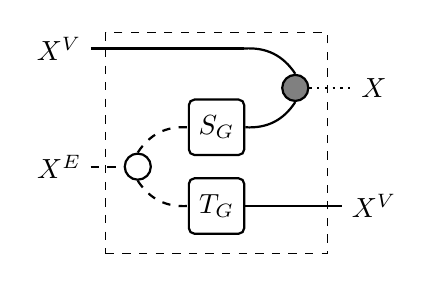
\begin{tikzpicture}
    \node[draw, circle, radius=5pt, thick] (copy) at (-1,0.5) {};
    \node[draw, minimum height=20, minimum width=20, rounded corners=2, thick] (S) at (0,1) {$S_G$};
    \node[draw, minimum height=20, minimum width=20, rounded corners=2, thick] (T) at (0,0) {$T_G$};
    \node[draw, fill=gray, circle, radius=5pt, thick] (mat) at (1,1.5) {};

    \node[draw, dashed, minimum height=80, minimum width=80] (contour) at (0,0.8) {};

    \node (Xv) at (-2,2) {$X^V$};
    \node (Xe) at (-2,0.5) {$X^E$};
    \node (X) at (2,1.5) {$X$};
    \node (Xv2) at (2,0) {$X^V$};

    \draw[-, thick] (Xv) to (10pt,2);
    \draw[bend left, thick] (10pt,2) to (mat.north);
    \draw[bend right, thick] (S.east) to (mat.south);

    \draw[dashed, -, thick] (Xe) to (copy.west);

    \draw[dashed, bend left, thick] (copy.north) to (S.west);
    \draw[dashed, bend right, thick] (copy.south) to (T.west);

    \draw[-, dotted, thick] (mat.east) -- (X);
    \draw[-, thick] (T.east) -- (Xv2.west);
  \end{tikzpicture}
\end{equation*}
%
%
\begin{theorem}\label{thm: path functor}
  Having chosen an enumeration on the vertexes and edges of a graph $G$, there 
  is a pseudofunctor $\Free{G} \to \Bkp$, sending 
  each object to $X^V$, and each generating morphism $e$ of $\Free{G}$ to the 
  following morphism, where $e$ represents the 
  constant gate outputting the enumeration of $e$ when considered as an edge of $G$:
  %
  %
  \begin{equation*}
    (\Id{X^V} \Tensor e);(\Id{X^V} \Tensor \COPYSym_{X^E});
      (\Id{X^V} \Tensor S_G \Tensor T_G);(\MATCHSym_{X^V} \Tensor \Id{X^V})
  \end{equation*}
  %
  %
  \begin{equation*}
    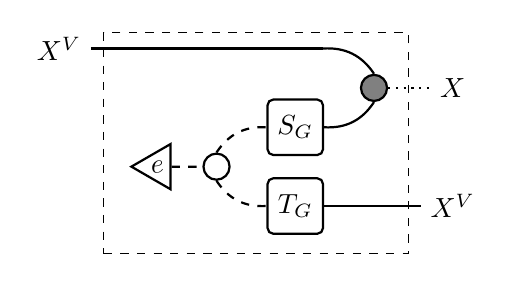
\begin{tikzpicture}
      \node[draw, circle, radius=5pt, thick] (copy) at (-1,0.5) {};
      \node[draw, minimum height=20, minimum width=20, rounded corners=2, thick] (S) at (0,1) {$S_G$};
      \node[draw, minimum height=20, minimum width=20, rounded corners=2, thick] (T) at (0,0) {$T_G$};
      \node[draw, fill=gray, circle, radius=5pt, thick] (mat) at (1,1.5) {};

      \node[draw, dashed, minimum height=80, minimum width=110] (contour) at (-0.5,0.8) {};

      \node (Xv) at (-3,2) {$X^V$};
      \node[draw, regular polygon, regular polygon sides = 3, rotate=-30, thick, label={[rotate=4]center:$e$}] (Xe) at (-1.75,0.5) {};
      \node (X) at (2,1.5) {$X$};
      \node (Xv2) at (2,0) {$X^V$};

      \draw[-, thick] (Xv) to (10pt,2);
      \draw[bend left, thick] (10pt,2) to (mat.north);
      \draw[bend right, thick] (S.east) to (mat.south);

      \draw[dashed, -, thick] (Xe) to (copy.west);

      \draw[dashed, bend left, thick] (copy.north) to (S.west);
      \draw[dashed, bend right, thick] (copy.south) to (T.west);

      \draw[-, dotted, thick] (mat.east) -- (X);
      \draw[-, thick] (T.east) -- (Xv2.west);
    \end{tikzpicture}
  \end{equation*}
  %
  %
  The image of $\Free{G}$ through this pseudofunctor is called 
  $\Bpath{G}$, the category of \emph{path proofs over $G$.}
\end{theorem}
%
The circuits of Theorem~\ref{thm: path functor} have the disadvantage of 
working on fixed paths, while we would like a general circuit 
working with every path of a given graph. To solve this problem, we take 
an intermediate step:
%
%
\begin{lemma}\label{lem: functor to count}
  Consider the category $\Count$, which has one object $*$ and 
  natural numbers as morphisms, with $0$ as the identity morphism 
  and composition as addition. 

  For each graph $G$, there is a functor $\Free{G} \to \Count$ sending 
  every object to  $*$, identities to $0$, and generating morphisms to $1$.
  This extends to a functorial correspondence between $\Graph$ and the 
  category of endofunctors over $\Count$.
\end{lemma}
%
$\Count$ is a category that, as the name suggests, counts how many 
generating morphisms compose a path. We can use it to shape general 
circuits that work for every path in a graph.
%
%
\begin{theorem}\label{thm: graph functor}
  For a graph $G$, consider an enumeration and $S_G$ and $T_G$ 
  as defined in Theorem~\ref{thm: path functor}. There is a pseudofunctor 
  $\Count \to \Bkp$ sending $*$ to $X^V$, $0$ to $\Id{X^V}$ 
  and $n > 0$ to the $n$-fold composition of the morphism
  %
  %
  \begin{equation*}
      (\Id{X^V} \Tensor \COPYSym_{X^E});
      (\Id{X^V} \Tensor S_G \Tensor T_G);(\MATCHSym_{X^V} \Tensor \Id{X^V})
  \end{equation*}
  %
  The composition of this pseudofunctor with the functor of 
  Lemma~\ref{lem: functor to count} gives a pseudofunctor 
  $\Free{G} \to \Count \to \Bkp$ sending each object to $X^V$, and each 
  generating morphism to the circuit:
  %
  %
  \begin{equation*}
    (\Id{X^V} \Tensor \COPYSym_{X^E});
      (\Id{X^V} \Tensor S_G \Tensor T_G);(\MATCHSym_{X^V} \Tensor \Id{X^V})
  \end{equation*}
  %
  %
  \begin{equation*}
    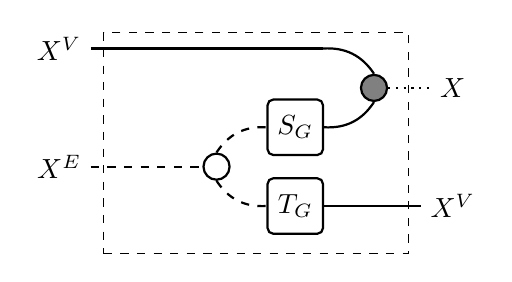
\begin{tikzpicture}
      \node[draw, circle, radius=5pt, thick] (copy) at (-1,0.5) {};
      \node[draw, minimum height=20, minimum width=20, rounded corners=2, thick] (S) at (0,1) {$S_G$};
      \node[draw, minimum height=20, minimum width=20, rounded corners=2, thick] (T) at (0,0) {$T_G$};
      \node[draw, fill=gray, circle, radius=5pt, thick] (mat) at (1,1.5) {};

      \node[draw, dashed, minimum height=80, minimum width=110] (contour) at (-0.5,0.8) {};

      \node (Xv) at (-3,2) {$X^V$};
      \node (Xe) at (-3,0.5) {$X^E$};
      \node (X) at (2,1.5) {$X$};
      \node (Xv2) at (2,0) {$X^V$};

      \draw[-, thick] (Xv) to (10pt,2);
      \draw[bend left, thick] (10pt,2) to (mat.north);
      \draw[bend right, thick] (S.east) to (mat.south);

      \draw[dashed, -, thick] (Xe) to (copy.west);

      \draw[dashed, bend left, thick] (copy.north) to (S.west);
      \draw[dashed, bend right, thick] (copy.south) to (T.west);

      \draw[-, dotted, thick] (mat.east) -- (X);
      \draw[-, thick] (T.east) -- (Xv2.west);
    \end{tikzpicture}
  \end{equation*}
  %
  The image of $\Free{G}$ through this pseudofunctor 
  is called $\Bgraph{G}$, the category of \emph{proofs over $G$.}
\end{theorem}
%
The pseudofunctor in Theorem~\ref{thm: graph functor} 
associates to each path of length $m$, seen as a morphism 
in $\Free{G}$, a generalized boolean circuit. 
This circuit accepts the enumeration of a vertex $v$ 
and a path of $n$ edges (specified as $n$ enumerations 
of edges) as inputs, and returns $1$ and an enumeration of $v'$
in output if the path leads from $v$ to $v'$. It returns $0$ and 
$\Zero$ otherwise. Notice that since we included identities 
in the truth tables when defining $S_G, T_G$, we are also 
able to verify \emph{any path of length less than $n$ by 
padding any path with identities}.
%
%
%
\subsection{Snarkizing circuits}
%
%
How do we turn the morphisms in 
$\Bgraph{G}$ into zk-SNARKS? 
Luckily enough, it turns out we do not have to build 
zk-SNARKS ourselves.  Indeed, there are already 
implemented ways to turn boolean circuits into 
zk-SNARKS~[]. Figuring out a cryptographically secure 
way to turn circuits into zk-SNARKS is no simple endeavour, 
that would probably take years and extensive security 
auditing. Instead, we deem a wiser course of action 
turning generalized boolean circuits in 
$\Bgraph{G}$ into boolean circuits, and feed them 
to an already implemented and audited solution.
%
%
\begin{definition}
  For each graph $G$ we define the \emph{snarkizator} as a function 
  $\Snark{\_} : \Mor{\Bgraph{G}} \to \Mor{\Bcirc}$ that 
  maps a morphism $f: X^V \to X^V$ to 
  %
  %
  \begin{equation*}
      (f \Tensor \Id{X^V});(\Id{X} \Tensor \MATCHSym_{X^V}); \ANDSym
  \end{equation*}
  %
  %
  \begin{equation*}
    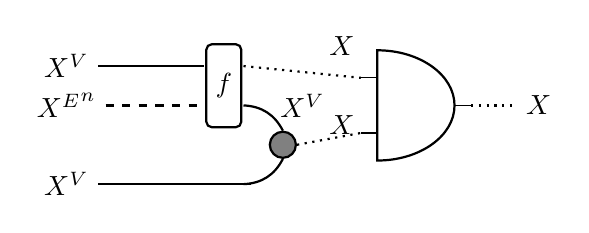
\begin{tikzpicture}
      \node[draw, minimum height=30, minimum width=5, rounded corners=2, thick] (f) at (0,1) {$f$};
      \node[draw, fill=gray, circle, radius=5pt, thick] (mat) at (0.75,0.25) {};
      \ctikzset{tripoles/american and port/input height=0.72};
      \ctikzset{tripoles/american and port/height=1};
      \ctikzset{tripoles/american and port/width=1};
      \node[american and port] (and) at (3,0.75) {};

      \node (Xv) at (-2,1.25) {$X^V$};
      \node (Xe) at (-2,0.75) {${X^E}^n$};
      \node (Xv2) at (-2,-0.25) {$X^V$};

      \node (X1) at (1.5,1.5) {$X$};
      \node (X2) at (1,0.75) {$X^V$};
      \node (X2) at (1.5,0.5) {$X$};

      \node (X3) at (4,0.75) {$X$};

      \draw[-, thick] (Xv) to (-0.25,1.25);
      \draw[dashed, -, thick] (Xe) to (-0.25,0.75);
      \draw[-, thick] (Xv2) to (10pt,-0.25);

      \draw[-, dotted, thick] (0.25, 1.25) -- (and.in 1);
      \draw[bend left, thick] (0.25,0.75) to (mat.north);

      \draw[bend right, thick] (0.25,-0.25) to (mat.south);
      \draw[-, dotted, thick] (mat.east) -- (and.in 2);

      \draw[-, dotted, thick] (and.out) -- (X3.west);
    \end{tikzpicture}
  \end{equation*}
  %
\end{definition}
%
Notice how a snarkized circuit just outputs a bit, and is 
thus a boolean circuit. Note moreover how the function 
$\Snark{\_}$ cannot be improved to a 
(pseudo)functor, since boolean circuits themselves 
do not form a category.

For each morphism $f$, $\Snark{f}$ is a boolean circuit which takes 
two values $a,b$ of type $X^V$ as input, representing vertexes, 
along with $f_1, \dots, f_n$ inputs of type $X^E$, representing 
edges, and returns $1$ if and only if the edge inputs define a valid path 
from $a$ to $b$ according to the graph specification defined by $S_G$ and $T_G$.
The corresponding zk-SNARK, obtained by simply feeding our circuit to 
any already available library such as \texttt{libsnark}~[], is a succint,
non-interactive zero knowledge proof that any specified 
path in the graph is valid or not.
%
%
%
\section{Abstracting over graphs}\label{sec: abstracting over graphs}
%
%
Up to now, circuits in~$\Bgraph{G}$ have the problem that 
the topology of $G$ is used to define $S_G$ and $T_G$, and is thus 
hardwired in the circuit. Since in creating zk-SNARKs some 
information has to be necessarily made public~[], this may cause 
problems. Indeed, it may be possible to reverse-engineer this 
public information to obtain information about $G$. Albeit 
this would still allow to keep used paths secret, the topology 
of the state space of a finite state machine can reveal a lot about 
what the finite state machine is used for. We would like to keep this 
information private.

To do this, we notice that as $S_G$ and $T_G$ are obtained by building 
a truth table from the adjacencies of $G$, this truth 
table could be fed itself to a ``universal function'' that builds $S$ and $T$
for all graphs up to a given size. In detail, if $n, m$ are numbers, 
we can consider boolean functions
%
%
\begin{equation*}
  \Source{m,n}{\_}, \Target{m,n}{\_}: \Bool^{f(m,n)} \times \Bool^m \to \Bool^n 
\end{equation*}
%
Which take $m$ bits in input, representing an enumeration of 
the edges of a graph whose source and target matrices are 
specified by $f(m,n)$ bits, and return $n$ bits, representing
an enumeration of their source and target, respectively. Notice how we 
write $f(m,n)$ since the size of the adjacency matrixes defining 
a graph will in general depend on the maximum number of 
vertexes and edges we are allowing. As before, we can 
invoke Theorem~\ref{thm: boolean circuits implement boolean 
functions} to consider implementations $S_{m,n}$ 
and $T_{m,n}$ of $\Source{m,n}{\_}$ and $\Target{m,n}{\_}$, 
respectively.

Since we have introduced new inputs, just substituting $S_{m,n}$ 
and $T_{m,n}$ in place of $S_G$ and $T_G$ in 
Theorems~\ref{thm: path functor} and~\ref{thm: graph functor}
won't work: Indeed, it would force us to specify the encoding
for $G$ $k$ times in a $k$-fold composition. Moreover, what happens 
if we give different graphs specifications in the composition?

The point is that the categorical structure 
of $\Bkp$ is not good to manage inputs that have to be 
routinely repeated. We fix these problems straight away 
by defining a new category as follows:
%
%
\begin{definition}\label{def: definition of bzkp}
  Fix a natural number $k$. We denote with $\Bzkp{k}$ 
  the \emph{bicategory of zero knowledge proof circuits of size $k$} defined 
  as follows:
  %
  %
  \begin{itemize}
    \item $\Obj{\Bzkp{k}} := \Obj{\Bcirc}$;
    %
    \item $\Mor{\Bzkp{k}}(A,B) := \Mor{\Bcirc}(A \Tensor X^k \Tensor X^n, X \Tensor B )$, for all $n \in \Naturals$.
    We depict morphisms as shown below; the $X^k$, $X^n$ and $X$ wires are ``silent'' with respect to 
    our categorical structure, so we depict them densely dotted, dashed and dotted, respectively:
    %
    %
    \begin{equation*}
    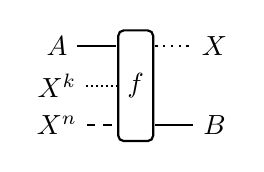
\begin{tikzpicture}
      \node[draw, minimum height=40, minimum width=5, rounded corners=2, thick] (f) at (-1,0.5) {$f$};
      \node (A) at (-2,1) {$A$};
      \node (Xk0) at (-2,0.5) {$X^{k}$};
      \node (Xn0) at (-2,0) {$X^{n}$};

      \node (Bf) at (0,1) {$X$};
      \node (B) at (0,0) {$B$};

      \draw[thick] (A) -- (-1.25,1);
      \draw[densely dotted,thick] (Xk0) -- (-1.25,0.5);
      \draw[dashed,thick] (Xn0) -- (-1.25,0);

      \draw[dotted,thick] (-0.75,1) -- (Bf);
      \draw[thick] (-0.75,0) -- (B);
    \end{tikzpicture}  
    \end{equation*}
    %
    \item $\Id{A} := \top \Tensor \Id{A} \Tensor \Id{X^k}: A \Tensor X^k \Tensor X^0  \to X \Tensor A$. Identites are
    depicted as follows:
    %
    %
    \begin{equation*}
    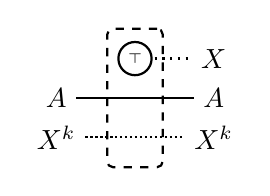
\begin{tikzpicture}
      \node[draw, dashed, minimum height=50, minimum width=20, rounded corners=2, thick] (f) at (-1,0.5) {};
      \node[thick, draw, circle, radius=2pt, inner sep = 2pt] (true) at (-1,1) {\tiny{$\top$}};
      \node (A) at (-2,0.5) {$A$};
      \node (Xk) at (-2,0) {$X^k$};

      \node (Bf) at (0,1) {$X$};
      \node (B) at (0,0.5) {$A$};
      \node (Xk2) at (0,0) {$X^k$};


      \draw[thick] (A) -- (B);
      \draw[densely dotted, thick] (Xk) -- (Xk2);

      \draw[dotted, thick] (-0.75,1) -- (Bf);
    \end{tikzpicture}  
    \end{equation*}
    %
    \item $\Mor{\Bzkp{1}}(A,B)(f,g) = \begin{cases}
      \{*\} & \text{ iff } \texttt{ext}(f) = \texttt{ext}(g);\\
      \,\,\,\, \emptyset & \text{ otherwise}
    \end{cases}$
    %
    \item Given $f : A \to B$ and $g: B \to C$, corresponding to 
    morphisms of $\Bcirc$ $A \Tensor X^{k} \Tensor X^{n_0} \to X \Tensor B$ and
    $B \Tensor X^{k} \Tensor X^{n_1} \to X \Tensor C$, respectively, 
    we set $f;g$ to be the morphism 
    %
    %
    \begin{equation*}
      (\Id{A} \Tensor \COPYSym_{X^k} \Tensor \Id{X^{n_0} \Tensor X^{n_1}});
      (\Id{A \Tensor X^{k}} \Tensor \sigma_{X^{n_0}, X^{k}} \Tensor \Id{X^{n_1}});
      (f \Tensor \Id{X^{k} \Tensor X^{n_1}});(\Id{X} \Tensor g);(\ANDSym \Tensor \Id{C})
    \end{equation*}
    %
    Where we denoted with $\sigma_{X^{n_0}, X^{k_1}}$
    the usual symmetries. Composition is depicted graphically as follows:
    %
    %
    \begin{equation*}
      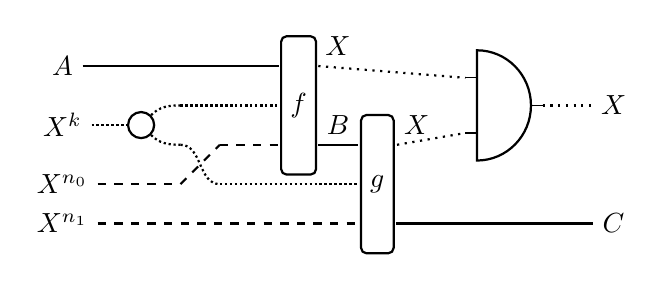
\begin{tikzpicture}
        \node[draw, circle, radius=1pt, thick] (copy) at (-3,1.25) {};
        \node[draw, minimum height=50, minimum width=5, rounded corners=2, thick] (f) at (-1,1.5) {$f$};
        \node[draw, minimum height=50, minimum width=5, rounded corners=2, thick] (g) at (0,0.5) {$g$};
        \ctikzset{tripoles/american and port/input height=0.7};
        \ctikzset{tripoles/american and port/height=1};
        \ctikzset{tripoles/american and port/width=.7};
        \node[american and port] (and) at (2,1.5) {};

        \node (A) at (-4,2) {$A$};
        \node (Xk) at (-4,1.25) {$X^{k}$};
        \node (Xn0) at (-4,0.5) {$X^{n_0}$};
        \node (Xn1) at (-4,-0) {$X^{n_1}$};

        \node (Bf) at (-0.5,2.25) {$X$};
        \node (B) at (-0.5,1.25) {$B$};
        \node (Bg) at (0.5,1.25) {$X$};
        \node (X) at (3,1.5) {$X$};
        \node (C) at (3,0) {$C$};
        
        \draw[thick] (A) -- (-1.25,2);
        \draw[densely dotted, thick] (Xk) -- (copy.west);
        \draw[dashed, thick] (Xn0) to (-2.5,0.5);
        \draw[dashed, thick] (Xn1) -- (-0.25,0);

        \draw[densely dotted, thick, out=45, in=180] (copy.north east) to (-2.5,1.5);
        \draw[densely dotted, thick, out=-45, in=180] (copy.south east) to (-2.5,1);

        \draw[densely dotted, thick, out=0, in=180] (-2.5,1.5) to (-1.25,1.5);
        \draw[densely dotted, thick, out=0, in=180] (-2.5,1) to (-2,0.5);
        \draw[dashed, thick] (-2.5,0.5) to (-2,1);

        \draw[dashed, thick] (-2,1) -- (-1.25,1);
        \draw[densely dotted, thick] (-2,0.5) -- (-0.25,0.5);

        \draw[dotted, thick] (-0.75,2) -- (and.in 1);
        \draw[thick] (-0.75,1) -- (-0.24, 1);
        \draw[dotted, thick] (0.25,1) -- (and.in 2);

        \draw[dotted, thick] (and.out) -- (X);
        \draw[thick] (0.24,0) -- (C);
      \end{tikzpicture}
    \end{equation*}
    %
    \item The 2-cell compositions and identities are trivial, and defined 
    in the obvious way.
  \end{itemize}
  %
\end{definition}%
%
Proceeding as in Lemma~\ref{lem: functor to count}, 
we are able to prove the following theorem:
%
%
\begin{theorem}\label{thm: bzkp functor}
  For each $n,m$, denote with $f(m,n)$ the function outputting how many
  bits are needed to store the source and target truth tables for graphs 
  with $n$ vertexes and $m$ edges. There is a functor $\Count \to \Bzkp{f(m,n)}$ sending each 
  number $k$ to the $k$-fold composition of the morphism
  %
  %
  \begin{equation*}
    (\Id{X^n} \Tensor \COPYSym_{X^{f(m,n)}} \Tensor \COPYSym_{X^m});
    (\Id{X^n \Tensor X^{f(m,n)}} \Tensor \sigma_{X^{f(m,n)},X^m} \Tensor \Id{X^m});
    (\Id{X^n} \Tensor S_{m,n} \Tensor T_{m,n});(\MATCHSym_{X^n} \Tensor \Id{X^n})
  \end{equation*}
  %
  %
  \begin{equation*}
    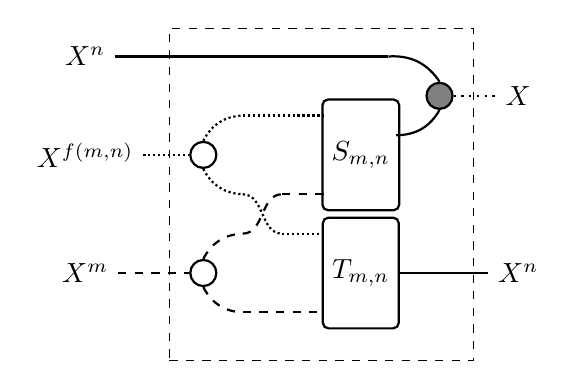
\begin{tikzpicture}
      \node[draw, circle, radius=5pt, thick] (copy2) at (-2,1.75) {};
      \node[draw, circle, radius=5pt, thick] (copy) at (-2,0.25) {};

      \node[draw, minimum height=40, minimum width=20, rounded corners=2, thick] (S) at (0,1.75) {$S_{m,n}$};
      \node[draw, minimum height=40, minimum width=20, rounded corners=2, thick] (T) at (0,0.25) {$T_{m,n}$};
      \node[draw, fill=gray, circle, radius=5pt, thick] (mat) at (1,2.5) {};

      \node[draw, dashed, minimum height=120, minimum width=110] (contour) at (-0.5,1.25) {};

      \node (Xv) at (-3.5,3) {$X^n$};
      \node (Xf) at (-3.5,1.75) {$X^{f(m,n)}$};
      \node (Xe) at (-3.5,0.25) {$X^m$};

      \node (X) at (2,2.5) {$X$};
      \node (Xv2) at (2,0.25) {$X^n$};

      \draw[-, thick] (Xv) to (10pt,3);
      \draw[-, densely dotted, thick] (Xf) to (copy2.west);
      \draw[-, dashed, thick] (Xe) to (copy.west);

      \draw[densely dotted, bend left, thick] (copy2.north) to (-1.5,2.25);
      \draw[densely dotted, bend right, thick] (copy2.south) to (-1.5, 1.25);
      \draw[dashed, bend left, thick] (copy.north) to (-1.5,0.75);
      \draw[dashed, bend right, thick] (copy.south) to (-1.5, -0.25);

      \draw[-, densely dotted, thick] (-1.5, 2.25) to (-0.47, 2.25);
      \draw[dashed, thick, out=0, in=180] (-1.5,0.75) to (-1, 1.25);
      \draw[densely dotted, thick, out=0, in=180] (-1.5,1.25) to (-1,0.75);
      \draw[-, dashed, thick] (-1.5, -0.25) to (-0.47,-0.25);

      \draw[-, dashed, thick] (-1, 1.25) to (-0.47, 1.25);
      \draw[-, densely dotted, thick] (-1, 0.75) to (-0.47,0.75);

      \draw[bend left, thick] (10pt,3) to (mat.north);
      \draw[bend right, thick] (0.45, 2) to (mat.south);

      \draw[dashed, -, thick] (Xe) to (copy.west);



      \draw[-, dotted, thick] (mat.east) -- (X);
      \draw[-, thick] (T.east) -- (Xv2.west);
    \end{tikzpicture}
  \end{equation*}
  %
\end{theorem}
%
Notice that Theorem~\ref{thm: bzkp functor} is stronger than 
one would expect: As in Theorem~\ref{thm: graph functor} we obtained
a circuit which not only verified a path of length $n$, but also all 
paths of smaller length for a given graph $G$, 
here we have something similar: $f(m,n)$ allows us to
feed  to the circuit the specification of \emph{any} graph
that has \emph{up to} $m$ edges and $n$ vertexes! In this sense, 
fixing $m,n$ amounts to fix some upper bounds for the size 
of the graphs, exactly as taking the $k$-fold composition of 
the circuit above amounts to fix some upper bound on the size 
of the computation we want to verify.
We conclude by putting everything together, showing how all the 
constructions we built behave well with respect to each other.
%
%
\begin{theorem}\label{thm: the cube}
Let $G$, $G'$ be graphs with $n, n'$ vertices and $m, m'$ 
edges, respectively. Denote with $f(n,m)$ the function 
outputting how many bits are needed to store the source 
and target truth tables for graphs with $n$ vertexes and $m$ edges. 
Then for each morphism $G \to G'$ the following diagram commutes:
%
\begin{equation*}
  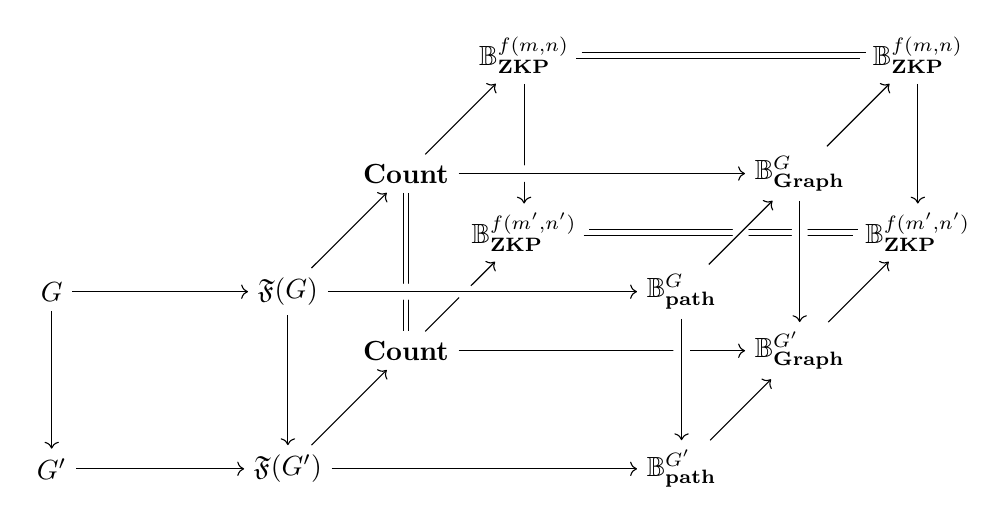
\begin{tikzpicture}
    \pgfdeclarelayer{fg}
    \pgfdeclarelayer{crossing}
    \pgfdeclarelayer{bg}
    \pgfsetlayers{main,bg,crossing,fg}
    %
    \node (G') at (0,0) {$G'$};
    \node(G) at (0,2.25) {$G$};
    \node(FG') at (3,0) {$\Free{G'}$};
    \node(FG) at (3,2.25) {$\Free{G}$};
    \node(Bpath') at (8,0) {$\Bpath{G'}$};
    \node(Bpath) at (8,2.25) {$\Bpath{G}$};
    \node(Count') at (4.5,1.5) {$\Count$};
    \node(Count) at (4.5,3.75) {$\Count$};
    \node(Bzkp') at (6,3) {$\Bzkp{f(m',n')}$};
    \node(Bzkp) at (6,5.25) {$\Bzkp{f(m,n)}$};
    \node(Bgraph') at (9.5,1.5) {$\Bgraph{G'}$};
    \node(Bgraph) at (9.5,3.75) {$\Bgraph{G}$};
    \node(Bzkp1') at (11,3) {$\Bzkp{f(m',n')}$};
    \node(Bzkp1) at (11,5.25) {$\Bzkp{f(m,n)}$};
    % Top
      \draw[->] (G) -- (FG);
      \draw[->] (FG) -- (Count);
      \draw[->] (Count) -- (Bzkp);
      \draw[transform canvas={yshift=-1pt, xshift=-1pt}, =] (Bzkp) -- (Bzkp1);
      \draw[transform canvas={yshift=1pt, xshift=1pt}, =] (Bzkp) -- (Bzkp1);
      \draw[->]  (Bgraph) -- (Bzkp1) ;
    % Bottom
      \draw[->] (G') -- (FG');
      \draw[->] (FG') -- (Bpath');
      \draw[->] (FG') -- (Count');
      \draw[->] (Bgraph') --  (Bzkp1');
      \draw[->] (Bpath') -- (Bgraph');
    % Vertical
      \draw[->] (G) -- (G');
      \draw[->] (FG) -- (FG');
      \draw[->] (Bzkp1) -- (Bzkp1');
    %FG
    \begin{pgfonlayer}{fg}
      \draw[->, name path global/.expanded=fgbpath] (FG) -- (Bpath);
      \draw[->, name path global/.expanded=countbgraph] (Count) -- (Bgraph);
      \draw[->, name path global/.expanded=bgraphbpath] (Bpath) -- (Bgraph);
      \draw[->, name path global/.expanded = bgraphbgraph'] (Bgraph) -- (Bgraph');
      \draw[->, name path global/.expanded=bpathbpath'] (Bpath) -- (Bpath');
    \end{pgfonlayer}
  %BG
    \begin{pgfonlayer}{bg}
      \draw[-> , name path global/.expanded=countbzkp'] (Count') -- (Bzkp');
      \draw[->, name path global/.expanded=countbgraph'] (Count') -- (Bgraph');
      \draw[transform canvas={yshift=-1pt, xshift=-1pt}, =, name path global/.expanded=bzkpid1] (Bzkp') -- (Bzkp1');
      \draw[transform canvas={yshift=1pt, xshift=1pt}, =, name path global/.expanded=bzkpid2] (Bzkp') -- (Bzkp1');
      \draw[transform canvas={xshift=-1pt}, =, name path global/.expanded=countcount'1] (Count) -- (Count');
      \draw[transform canvas={xshift=1pt}, =, name path global/.expanded=countcount'2] (Count) -- (Count');
      \draw[->, name path=bzkpbzkp'] (Bzkp) -- (Bzkp');
    \end{pgfonlayer}
    % Intersections
    \begin{pgfonlayer}{crossing}
      \fill[white, name intersections={of=bgraphbpath and bzkpid1, name=i}] (i-1) circle (3pt);
      \fill[white, name intersections={of=bgraphbpath and bzkpid2, name=i}] (i-1) circle (3pt);
      \fill[white, name intersections={of=bgraphbgraph' and bzkpid1, name=i}] (i-1) circle (3pt);
      \fill[white, name intersections={of=bgraphbgraph' and bzkpid2, name=i}] (i-1) circle (3pt);
      \fill[white, name intersections={of=fgbpath and countbzkp', name=i}] (i-1) circle (3pt);
      \fill[white, name intersections={of=countbgraph' and bpathbpath', name=i}] (i-1) circle (3pt);
      \fill[white, name intersections={of=bzkpbzkp' and countbgraph, name=i}] (i-1) circle (3pt);
      \fill[white, name intersections={of=countcount'1 and fgbpath, name=i}] (i-1) circle (3pt);
      \fill[white, name intersections={of=countcount'2 and fgbpath, name=i}] (i-1) circle (3pt);
    \end{pgfonlayer}
    %
    \end{tikzpicture}
  %
\end{equation*}
%
\end{theorem}
%
%
\section{Conclusion and future work}\label{sec: conclusion}
%
%
We defined a pseudofunctorial way to turn graphs into families of 
boolean circuits that can verify the correctness of any path in the graph.
Then, we generalized this to circuits that can verify correctness of 
paths for any graph with a bounded number of vertexes and edges, 
obtaining a pseudofunctorial correspondence between 
the category $\Graph$ and the category of circuits [].

Since graphs can be used to represent finite state machines and 
boolean circuits can be compiled into zk-SNARKS, this in turn 
provides a pseudofunctorial way to turn FSMs into zk-SNARKS.

Ongoing work includes implementing our correspondence in a 
formally verified setting using dependent types. Future work is 
mainly focused in generalizing our machinery to map free symmetric
strict monoidal categories into boolean circuits, providing a way to 
define arbitrary executions for Petri nets.
%
%
%
\section*{Acknowledgements}
The authors want to thank the Ehtereum Foundation, 
that financed this work with a grant.

%QPL Wants Bibtex!
%
%\printbibliography 
%\newpage
%

\bibliographystyle{eptcs}
\bibliography{bibtexbibliography}

\clearpage
\appendix
\section*{Appendix - Proofs}
%
%
\begingroup
\def\thetheoremUnified{\ref{lem: monoidal functor Bcirc Bfun}}
\begin{theorem}
  There is a strict monoidal functor $\texttt{ext}: \Bcirc \to \Bfun$ sending
  $I$ to $\Bool^0$, $X$ to $\Bool$, $\NANDSym$ to the usual 
  \texttt{NAND} function $\Bool^2 \to \Bool$, $\COPYSym$ to the 
  cartesian diagonal on $\Bool$, and $\top, \bot$ to the 
  functions $\Bool^0 \to \Bool$ corresponding to the constants 
  $1$ and $0$, respectively.
\end{theorem}
\addtocounter{theoremUnified}{-1}
\endgroup
\begin{proof}
  Strict monoidal functoriality is obvious from the freeness of $\Bcirc$.
\end{proof}
%
%
\begin{lemma}\label{lem: bkp is a bicategory}
  $\Bkp$ as defined in Definition~\ref{def: definition of bkp} is a bicategory.
\end{lemma}
\begin{proof}
  First notice that for each $A,B$, $\Bkp(A,B)$ is trivially a category, 
  since function extensionality is reflexive and transitive.

  Moreover, composition is clearly functorial. This follows from the fact 
  that extensionality is a congruence with respect to function composition.

  The existence of unitors and associators follows from the fact that 
  $\ANDSym(x, 1)$ and $\ANDSym(1,x)$ are extensionally equal to the 
  identity function $\Bool \to \Bool$, as extensionally equal are 
  $\ANDSym(\ANDSym(\_,\_),\_)$ and $\ANDSym(\_,\ANDSym(\_,\_))$.

  Naturality and satisfaction of pentagon and triangle identities for 
  associators and unitors, respectively, follows from the 
  fact that the 2-cell structure of $\Bkp$ is posetal, so proving 
  that such morphisms exist is enough.
\end{proof}
%
%
\begingroup
\def\thetheoremUnified{\ref{thm: path functor}}
\begin{theorem}
  Having chosen an enumeration on the vertexes and edges of a graph $G$, there 
  is a pseudofunctor $\Free{G} \to \Bkp$, sending 
  each object to $X^V$, and each generating morphism $e$ of $\Free{G}$ to the 
  following morphism, called \emph{$e$-evaluator}, where $e$ represents the 
  constant gate outputting the enumeration of $e$ when considered as an edge of $G$:
  %
  %
  \begin{equation*}
    (\Id{X^V} \Tensor e);(\Id{X^V} \Tensor \COPYSym_{X^E});
      (\Id{X^V} \Tensor S_G \Tensor T_G);(\MATCHSym_{X^V} \Tensor \Id{X^V})
  \end{equation*}
  %
  %
  \begin{equation*}
    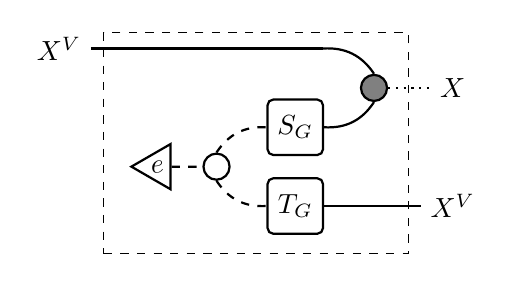
\begin{tikzpicture}
      \node[draw, circle, radius=5pt, thick] (copy) at (-1,0.5) {};
      \node[draw, minimum height=20, minimum width=20, rounded corners=2, thick] (S) at (0,1) {$S_G$};
      \node[draw, minimum height=20, minimum width=20, rounded corners=2, thick] (T) at (0,0) {$T_G$};
      \node[draw, fill=gray, circle, radius=5pt, thick] (mat) at (1,1.5) {};

      \node[draw, dashed, minimum height=80, minimum width=110] (contour) at (-0.5,0.8) {};

      \node (Xv) at (-3,2) {$X^V$};
      \node[draw, regular polygon, regular polygon sides = 3, rotate=-30, thick, label={[rotate=4]center:$e$}] (Xe) at (-1.75,0.5) {};
      \node (X) at (2,1.5) {$X$};
      \node (Xv2) at (2,0) {$X^V$};

      \draw[-, thick] (Xv) to (10pt,2);
      \draw[bend left, thick] (10pt,2) to (mat.north);
      \draw[bend right, thick] (S.east) to (mat.south);

      \draw[dashed, -, thick] (Xe) to (copy.west);

      \draw[dashed, bend left, thick] (copy.north) to (S.west);
      \draw[dashed, bend right, thick] (copy.south) to (T.west);

      \draw[-, dotted, thick] (mat.east) -- (X);
      \draw[-, thick] (T.east) -- (Xv2.west);
    \end{tikzpicture}
  \end{equation*}
  %
  %
  The image of $\Free{G}$ through this pseudofunctor is called 
  $\Bpath{G}$, the category of \emph{path proofs over $G$.}
\end{theorem}
\addtocounter{theoremUnified}{-1}
\endgroup
\begin{proof}
  Obvious from the freeness of $\Free{G}$ and the fact that the 
  bicategorical structure of $\Bkp$ is trivial.
\end{proof}
%
%
\begingroup
\def\thetheoremUnified{\ref{thm: path functor}}
\begin{lemma}
  Consider the category $\Count$, which has one object $*$ and 
  natural numbers as morphisms, with $0$ is the identity morphism 
  and composition as addition. 

  For each graph $G$, there is a pseudofunctor $\Free{G} \to \Count$ sending 
  every object to  $*$, identities to $0$, and generating morphisms to $1$.
  This extends to a functorial correspondence between $\Graph$ and the 
  category of endofunctors over $\Count$.
\end{lemma}
\addtocounter{theoremUnified}{-1}
\endgroup
\begin{proof}
  Functoriality is obvious from the freeness of $\Free{G}$.
\end{proof}
%
%
\begingroup
\def\thetheoremUnified{\ref{thm: graph functor}}
\begin{theorem}
  For a graph $G$, consider an enumeration and $S_G$ and $T_G$ 
  as defined in Theorem~\ref{thm: path functor}. There is a pseudofunctor 
  $\Count \to \Bkp$ sending $*$ to $X^V$, $0$ to $\Id{X^V}$ 
  and $n > 0$ to the $n$-fold composition of the morphism
  %
  %
  \begin{equation*}
      (\Id{X^V} \Tensor \COPYSym_{X^E});
      (\Id{X^V} \Tensor S_G \Tensor T_G);(\MATCHSym_{X^V} \Tensor \Id{X^V})
  \end{equation*}
  %
  The composition of this pseudofunctor with the pseudofunctor of 
  Lemma~\ref{lem: functor to count} gives a pseudofunctor 
  $\Free{G} \to \Count \to \Bkp$ sending each object to $X^V$, and each 
  generating morphism to the circuit:
  %
  %
  \begin{equation*}
    (\Id{X^V} \Tensor \COPYSym_{X^E});
      (\Id{X^V} \Tensor S_G \Tensor T_G);(\MATCHSym_{X^V} \Tensor \Id{X^V})
  \end{equation*}
  %
  %
  \begin{equation*}
    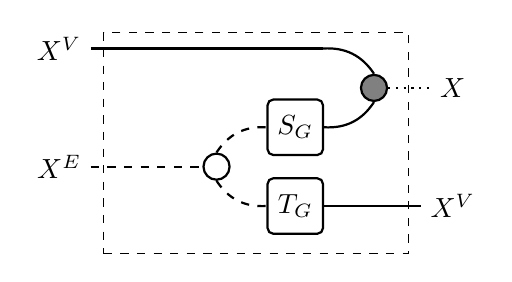
\begin{tikzpicture}
      \node[draw, circle, radius=5pt, thick] (copy) at (-1,0.5) {};
      \node[draw, minimum height=20, minimum width=20, rounded corners=2, thick] (S) at (0,1) {$S_G$};
      \node[draw, minimum height=20, minimum width=20, rounded corners=2, thick] (T) at (0,0) {$T_G$};
      \node[draw, fill=gray, circle, radius=5pt, thick] (mat) at (1,1.5) {};

      \node[draw, dashed, minimum height=80, minimum width=110] (contour) at (-0.5,0.8) {};

      \node (Xv) at (-3,2) {$X^V$};
      \node (Xe) at (-3,0.5) {$X^E$};
      \node (X) at (2,1.5) {$X$};
      \node (Xv2) at (2,0) {$X^V$};

      \draw[-, thick] (Xv) to (10pt,2);
      \draw[bend left, thick] (10pt,2) to (mat.north);
      \draw[bend right, thick] (S.east) to (mat.south);

      \draw[dashed, -, thick] (Xe) to (copy.west);

      \draw[dashed, bend left, thick] (copy.north) to (S.west);
      \draw[dashed, bend right, thick] (copy.south) to (T.west);

      \draw[-, dotted, thick] (mat.east) -- (X);
      \draw[-, thick] (T.east) -- (Xv2.west);
    \end{tikzpicture}
  \end{equation*}
  %
  The image of $\Free{G}$ through this pseudofunctor 
  is called $\Bgraph{G}$, the category of \emph{proofs over $G$.}
\end{theorem}
\addtocounter{theoremUnified}{-1}
\endgroup
\begin{proof}
  The only non-trivial part is proving pseudofunctoriality 
  of the functor $\Count \to \Bkp$. For this, notice that 
  the same natural number $n$ can be obtained by 
  adding smaller numbers in different orders, and with 
  different bracketings. These will in turn correspond to 
  different ways to compose the same morphism in $\Bkp$,
  $n$-times. All these compositions are extensionally equal, 
  which guarantees the existence of isomorphic 2-cells between 
  them. Pseudofunctoriality follows trivially, leveraging on the 
  fact that the 2-cell structure of $\Bkp$ is itself trivial.
\end{proof}
%
%
\begin{lemma}
  For each $n$, $\Bzkp{n}$ as defined in Definition~\ref{def: definition of bzkp} is a bicategory.
\end{lemma}
\begin{proof}
  The proof proceeds exactly as in Lemma~\ref{lem: bkp is a bicategory}, 
  by applying function extensionality also to different 
  compositions of $\COPYSym_X^m$  and $\sigma_{X^{f(n,m)},X^m}$.
\end{proof}
%
%
\begingroup
\def\thetheoremUnified{\ref{thm: the cube}}
\begin{theorem}
  Let $G$, $G'$ be graphs with $n, n'$ vertices and $m, m'$ edges, respectively. 
  Then for each morphism $G \to G'$ and each path $p$ of $G$ the following diagram commutes:
  %
\begin{equation*}
  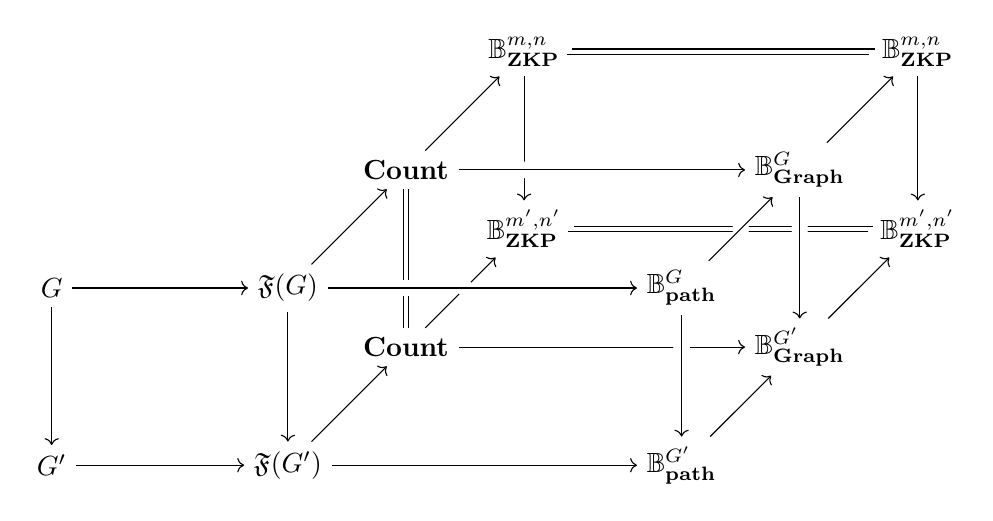
\begin{tikzpicture}
    \pgfdeclarelayer{fg}
    \pgfdeclarelayer{crossing}
    \pgfdeclarelayer{bg}
    \pgfsetlayers{main,bg,crossing,fg}
    %
    \node (G') at (0,0) {$G'$};
    \node(G) at (0,2.25) {$G$};
    \node(FG') at (3,0) {$\Free{G'}$};
    \node(FG) at (3,2.25) {$\Free{G}$};
    \node(Bpath') at (8,0) {$\Bpath{G'}$};
    \node(Bpath) at (8,2.25) {$\Bpath{G}$};
    \node(Count') at (4.5,1.5) {$\Count$};
    \node(Count) at (4.5,3.75) {$\Count$};
    \node(Bzkp') at (6,3) {$\Bzkp{m',n'}$};
    \node(Bzkp) at (6,5.25) {$\Bzkp{m,n}$};
    \node(Bgraph') at (9.5,1.5) {$\Bgraph{G'}$};
    \node(Bgraph) at (9.5,3.75) {$\Bgraph{G}$};
    \node(Bzkp1') at (11,3) {$\Bzkp{m',n'}$};
    \node(Bzkp1) at (11,5.25) {$\Bzkp{m,n}$};
    % Top
      \draw[->] (G) -- (FG);
      \draw[->] (FG) -- (Count);
      \draw[->] (Count) -- (Bzkp);
      \draw[transform canvas={yshift=-1pt, xshift=-1pt}, =] (Bzkp) -- (Bzkp1);
      \draw[transform canvas={yshift=1pt, xshift=1pt}, =] (Bzkp) -- (Bzkp1);
      \draw[->]  (Bgraph) -- (Bzkp1) ;
    % Bottom
      \draw[->] (G') -- (FG');
      \draw[->] (FG') -- (Bpath');
      \draw[->] (FG') -- (Count');
      \draw[->] (Bgraph') --  (Bzkp1');
      \draw[->] (Bpath') -- (Bgraph');
    % Vertical
      \draw[->] (G) -- (G');
      \draw[->] (FG) -- (FG');
      \draw[->] (Bzkp1) -- (Bzkp1');
    %FG
    \begin{pgfonlayer}{fg}
      \draw[->, name path global/.expanded=fgbpath] (FG) -- (Bpath);
      \draw[->, name path global/.expanded=countbgraph] (Count) -- (Bgraph);
      \draw[->, name path global/.expanded=bgraphbpath] (Bpath) -- (Bgraph);
      \draw[->, name path global/.expanded = bgraphbgraph'] (Bgraph) -- (Bgraph');
      \draw[->, name path global/.expanded=bpathbpath'] (Bpath) -- (Bpath');
    \end{pgfonlayer}
  %BG
    \begin{pgfonlayer}{bg}
      \draw[-> , name path global/.expanded=countbzkp'] (Count') -- (Bzkp');
      \draw[->, name path global/.expanded=countbgraph'] (Count') -- (Bgraph');
      \draw[transform canvas={yshift=-1pt, xshift=-1pt}, =, name path global/.expanded=bzkpid1] (Bzkp') -- (Bzkp1');
      \draw[transform canvas={yshift=1pt, xshift=1pt}, =, name path global/.expanded=bzkpid2] (Bzkp') -- (Bzkp1');
      \draw[transform canvas={xshift=-1pt}, =, name path global/.expanded=countcount'1] (Count) -- (Count');
      \draw[transform canvas={xshift=1pt}, =, name path global/.expanded=countcount'2] (Count) -- (Count');
      \draw[->, name path=bzkpbzkp'] (Bzkp) -- (Bzkp');
    \end{pgfonlayer}
    % Intersections
    \begin{pgfonlayer}{crossing}
      \fill[white, name intersections={of=bgraphbpath and bzkpid1, name=i}] (i-1) circle (3pt);
      \fill[white, name intersections={of=bgraphbpath and bzkpid2, name=i}] (i-1) circle (3pt);
      \fill[white, name intersections={of=bgraphbgraph' and bzkpid1, name=i}] (i-1) circle (3pt);
      \fill[white, name intersections={of=bgraphbgraph' and bzkpid2, name=i}] (i-1) circle (3pt);
      \fill[white, name intersections={of=fgbpath and countbzkp', name=i}] (i-1) circle (3pt);
      \fill[white, name intersections={of=countbgraph' and bpathbpath', name=i}] (i-1) circle (3pt);
      \fill[white, name intersections={of=bzkpbzkp' and countbgraph, name=i}] (i-1) circle (3pt);
      \fill[white, name intersections={of=countcount'1 and fgbpath, name=i}] (i-1) circle (3pt);
      \fill[white, name intersections={of=countcount'2 and fgbpath, name=i}] (i-1) circle (3pt);
    \end{pgfonlayer}
    %
    \end{tikzpicture}
  %
\end{equation*}
%
\end{theorem}
\addtocounter{theoremUnified}{-1}
\endgroup
\begin{proof}
  TODO
\end{proof}

\end{document}
